\documentclass[12pt]{scrreprt}
\usepackage{xeCJK}
\usepackage{amsmath, amssymb, amsthm, bm}
\usepackage{graphicx}
\usepackage[margin=2.5cm]{geometry}
\usepackage{rotating}
\usepackage{makeidx}
\usepackage{psfrag}
\usepackage{epsf}
\usepackage{epsfig}
\usepackage{stfloats}
\usepackage{subfig}
%\usepackage{array}
\usepackage{amsfonts} % Needed for blackboard bold, etc
\usepackage{amssymb} % a superset of amsfonts
\usepackage{url}
\usepackage{psfrag,calc,url,bm}
\usepackage{graphicx,booktabs,color}
\usepackage{stfloats}
\usepackage[]{algorithm}
\usepackage{svg}
\usepackage{tikz}
\usetikzlibrary{arrows.meta, positioning}
\usepackage{adjustbox} % for scaling
\usepackage{algpseudocode}
\usepackage[]{cite}
\newcommand\Wb{\ensuremath{{\bf W}}}
\newcommand\vb{\ensuremath{{\bf v}}}
\newcommand\wb{\ensuremath{{\bm w}}}
\newcommand\hb{\ensuremath{{\bf h}}}
\newcommand\xb{\ensuremath{{\bf x}}}
\newcommand\tr{\ensuremath{{\bf Tr}}}
\newcommand\nub{\bm{\nu}}
\newcommand\zerob{\ensuremath{{\bf 0}}}



	
\title{{\textbf \LARGE National Tsing Hua University}\\[1.5cm]

\Large{Error Correcting Codes II} \\[1.5cm]

\Large{\normalfont Final Project Report}\\[1.5cm]


\includegraphics[scale=2.5]{nthu_logo}\\[1.5cm]

\Large{Rate 1/2-LDPC Code Simulation}\\[1cm] }

\author{\large Njini Nathan Fofeyin \\[0.5cm] 112064422 \\[0.5cm] 恩哲倪}

\date{\large \today}

\begin{document}
		
	\begin{titlepage}
		\maketitle
		
		\chapter*{\Large Abstract}
		This report presents the simulation and performance evaluation of a WiMAX-style Low-Density Parity-Check (LDPC) code with a rate of 1/2 and a codeword length of 2304 bits. The encoder is implemented using a double-diagonal parity construction with an expansion factor $Z = 96$, based on a standardized $12 \times 24$ base matrix. Decoding is performed using the log-domain Sum-Product Algorithm (log-SPA) with the $\phi(\cdot)$ function approximation for improved numerical stability. The minsum algorithm is laso implemented. The simulations are conducted over an additive white Gaussian noise (AWGN) channel using binary phase-shift keying (BPSK) modulation. Bit error rate (BER) performance is analyzed across a range of signal-to-noise ratios (SNRs), demonstrating the error-correcting capability of the code. The results validate the expected coding gain and confirm the effectiveness of the log-SPA decoder implementation and minsum algorithm.
		
	\end{titlepage}
	
	\tableofcontents
	\addcontentsline{toc}{chapter}{Abstract}
	
	\chapter{Introduction}
	LDPC Codes were first introduced by Robert Gallager in 1960. Since then, they have been adopted into several technology standards. In this project, an LDPC code simulation is completed. The code is from the WiMaX (IEEE 802.16e) standard, and it consists of several properties that makes it suitable and efficient for error correction and reliable channel coding \cite{rptu}.
	
	In this project, we primarily consider the log domain sum product algorithm (hereafter referred to as log SPA) to study the bit error rate (BER) performance for a rate 1/2 $(m, n)$-LDPC code where $m = 1152$ and $n = 2304$. As is common for LDPC codes in standards such as 5G NR, WiFi (IEEE 802.11n), satellite communication and WiMaX, our code design has a special structure, completely characterized by $({\mathbf B}, Z, {\mathbf I}_{Z}, \text{rate})$, where ${\mathbf B}$ is the base matrix (also known as protograph), the expansion factor $Z$, ${\mathbf I}_{Z}$ is a $ Z \times Z $ identity matrix, with rate representing the fraction of message bits to the entire codeword. 
	
	These parameters can be used to directly construct the parity check matrix ${\mathbf H}$ of the code which can be used primarily for decoding codewords. In our given code, the ${\mathbf H}$ matrix has a special double diagonal structure. In the next section, we will discuss the implications of this structure for encoding, eliminating the need for a generator matrix ${\mathbf G}$ for the encoding process.
	
	In this project, we realize a complete end-to-end simulation of $1152 \times 2304$ LDPC code of rate 1/2 was simulated and the BER performance over an AWGN channel using both the log SPA algorithms and minsum algorithms. We perform this simulation using monte carlo method by randomly generating a large number of random bits and performing the simulation until we have a converged BER rate. We utilize a fairly large number of code words (\verb|max_num_rounds <= 150000|). We significantly reduce the amount of simulation time required to perform the simulation by checking for convergence of the BER to the mean of the previous \verb|100| BER values. We deem this value appropriate for this simulation, and ensure that at least a confidence interval of 0.95 is achieved. Elaborate details are provided in section 5.
	
	Each of 3 blocks are carefully modelled and implemented to realize the simulation. These include the encoder, channel and decoder as shown in figure \ref{fig:system}. Each of these play the following roles:

	\begin{figure}[htbp]
	\centering
	\begin{adjustbox}{width=\textwidth, padding=10pt} % adds spacing around
		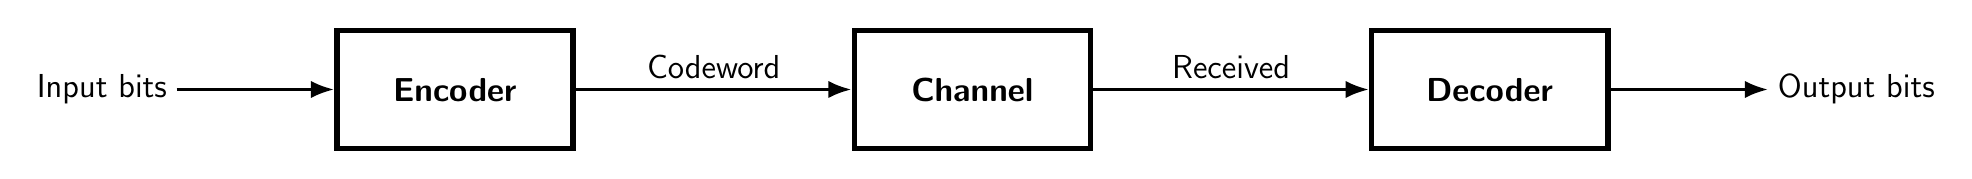
\begin{tikzpicture}[>=Latex, node distance=3.5cm, every node/.style={font=\sffamily\large}]
			% Nodes with thicker borders and bigger min size
			\node[draw, line width = 2pt, minimum width=3cm, minimum height=1.5cm] (enc) {\textbf{Encoder}};
			\node[draw, line width = 2pt, right=of enc, minimum width=3cm, minimum height=1.5cm] (chan) {\textbf{Channel}};
			\node[draw, line width = 2pt, right=of chan, minimum width=3cm, minimum height=1.5cm] (dec) {\textbf{Decoder}};
			
			% Labels and arrows with thicker lines and bigger text
			\node[left=2cm of enc, font=\sffamily\large] (input) {Input bits};
			\node[right=2cm of dec, font=\sffamily\large] (output) {Output bits};
			
			\draw[->, very thick] (input) -- (enc);
			\draw[->, very thick] (enc) -- node[above, font=\sffamily\large]{Codeword} (chan);
			\draw[->, very thick] (chan) -- node[above, font=\sffamily\large]{Received} (dec);
			\draw[->, very thick] (dec) -- (output);
		\end{tikzpicture}
	\end{adjustbox}
	\caption{End-to-end simulation framework.}
	\label{fig:system}
\end{figure}


	\begin{enumerate}
		\item \textbf{Encoder:} Maps input message bits to a codeword using the LDPC parity check matrix ${\mathbf H}$. This is achieved using the dual diagonal encoding technique.
		\item \textbf{Channel:} Introduces noise or distortions modeled by a specific channel model (e.g., AWGN, Rayleigh, BSC etc). In our case, we utilize a BI-AWGNC $\mathcal{N}(0,\sigma^2)$, where sigma is the channel's noise variance.
		\item \textbf{Decoder:} Estimates transmitted codeword bits from noisy observations using a decoding algorithm such as log SPA, or minsum. These are generally referred to as belief propagation algorithms.
	\end{enumerate}

	It is worth noting that from the codeword, the decoded message bits can then be directly extracted depending on the rate and encoding technique. In our case, we obtain the message by directly grabbing the first half bits from the decoded codeword due to systematic encoding and our code rate $r = \frac{1}{2}$. This is also possible due to no interleaving in the encoding step. The number of message bits is determined by the code rate.
	
	We establish that the code is capable of achieving low error rates of the order $\sim 10^{-5}$ to $\sim 10^{-7}$ for high SNR. These statistical estimates are obtained by simulating a large number of bits until a converged BER value is obtained.
	
	\chapter{Encoder}
	\section{Code Construction}
	The parity check matrix ${\mathbf H}$ completely characterizes an LDPC code. In standards, this is usually constructed from a so-called base matrix (protograph). In our case, the base matrix ${\mathbf B}$ is given as follows 

	\begin{figure}[htbp]
		\makebox[\linewidth][c]{%
			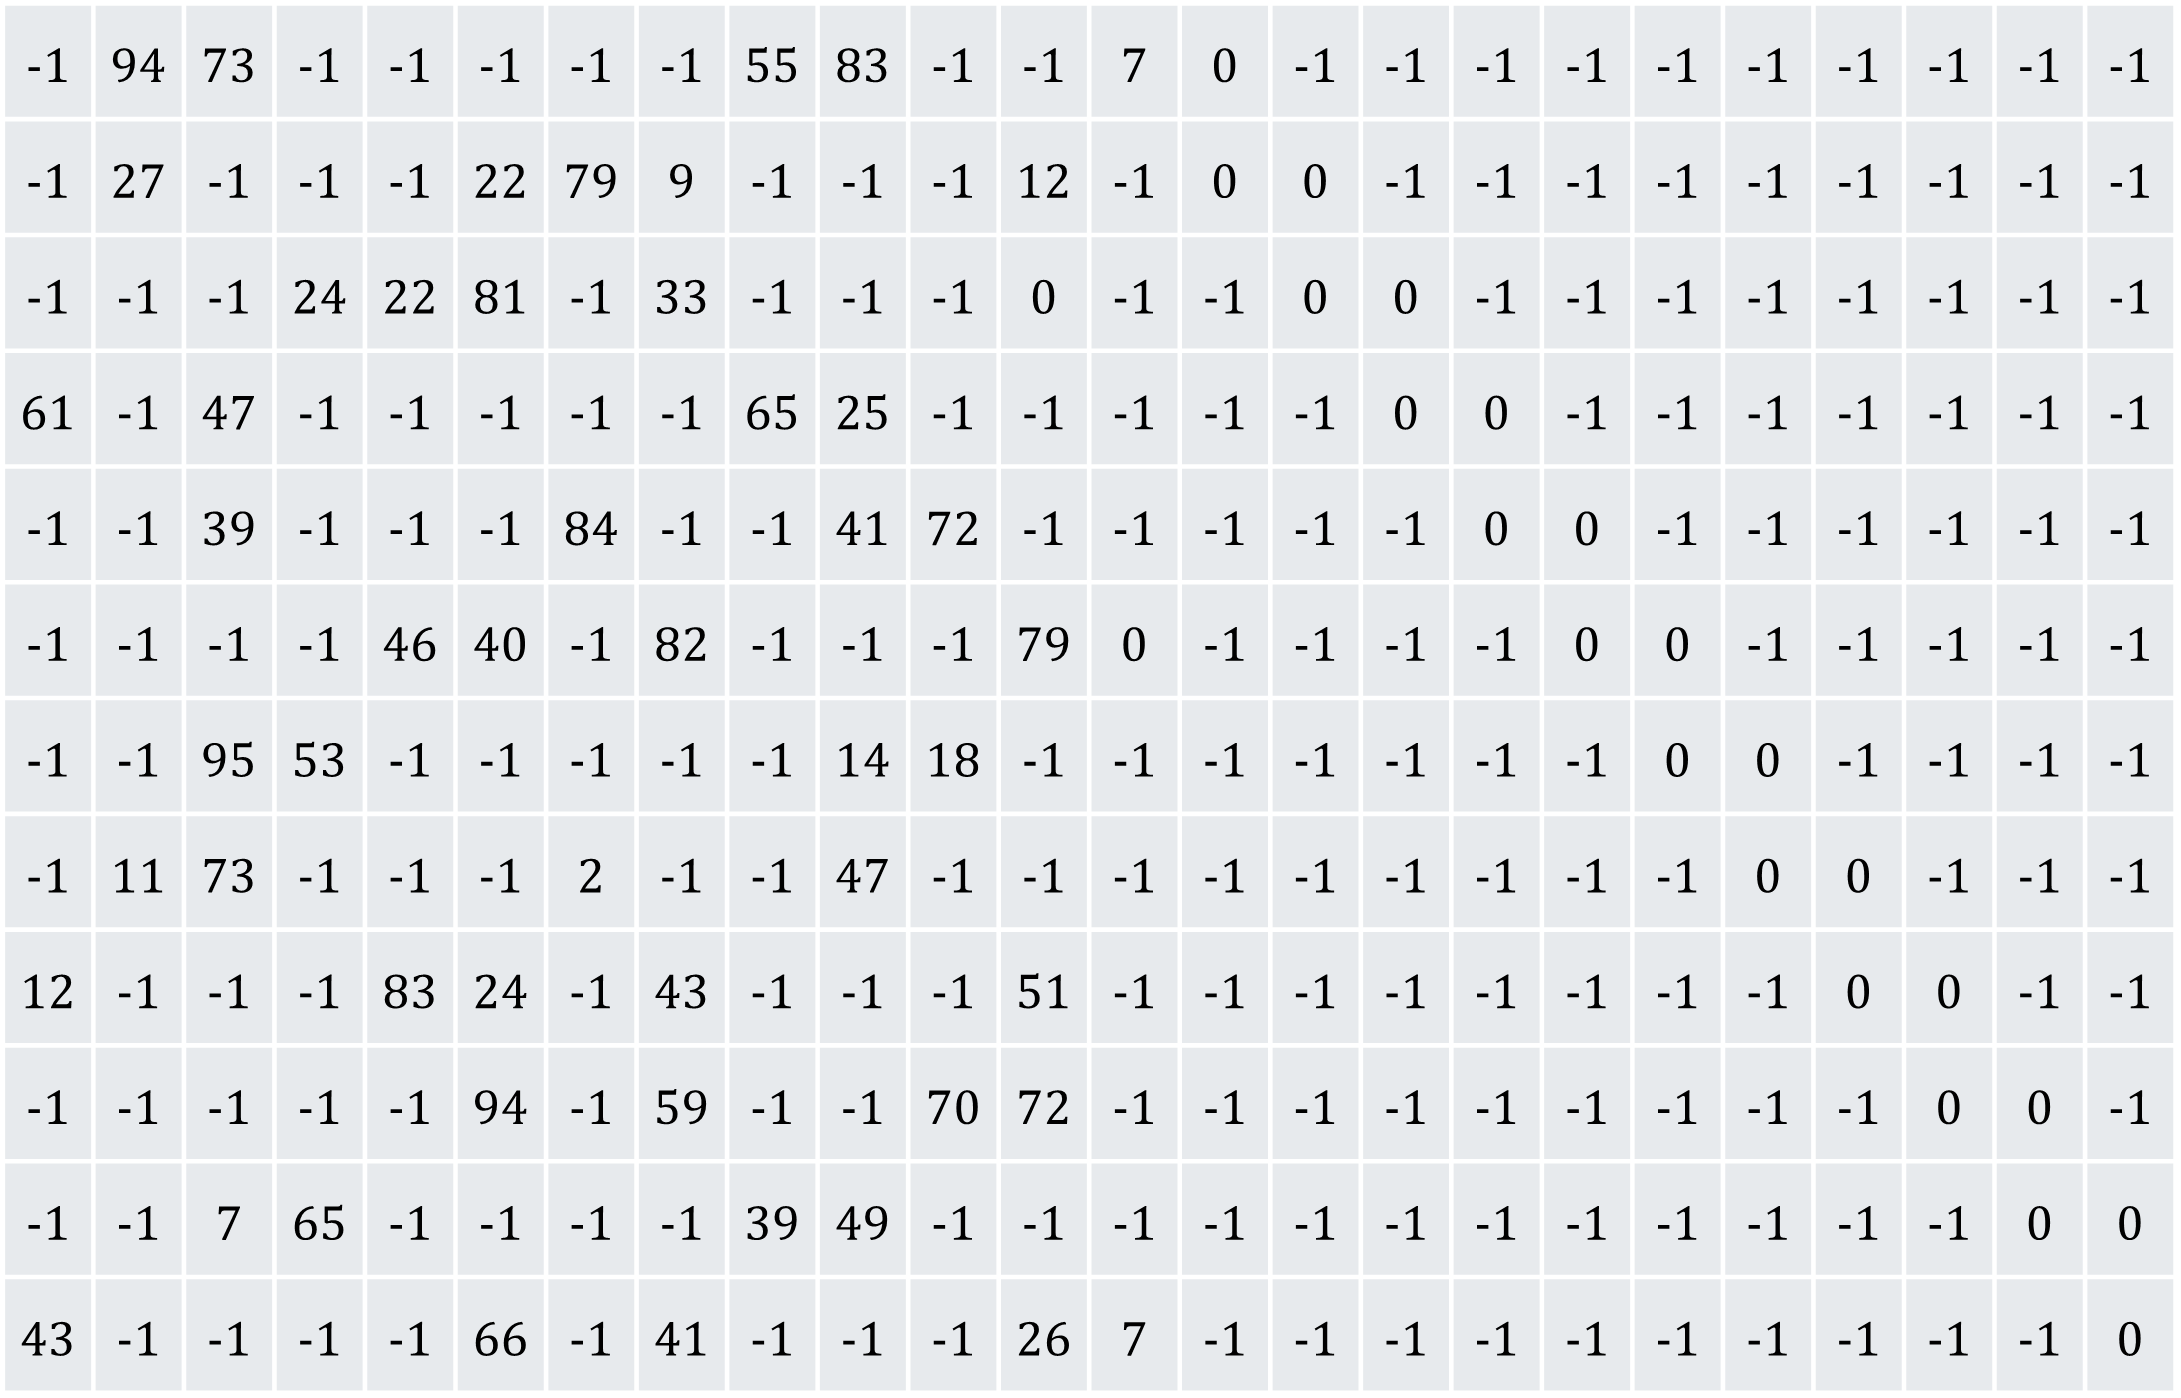
\includegraphics[width=0.75\textwidth, height=\textheight, keepaspectratio]{base_matrix}
		}
		\caption{Base Matrix, ${\mathbf B}$ }
		\label{fig:base_matrix}
	\end{figure}
	The base matrix indicates shifting coefficients such that the resulting parity matrix is sparse and irregular LDPC code. The resulting code is a quasi-cyclic LDPC code since each identity matrix block $\mathbf{I}_{96 \times 96}$ has shifted columns. The shifting mechanism is designed to make the matrix sparse and to generate seemingly random codes towards achieving channel capacity. It is also designed to avoid short cycles in the Tanner graph, which can affect decoding performance, especially for BEC channels (although not a major concern for this project).
	
	\begin{figure}[H]
		\makebox[\linewidth][c]{%
			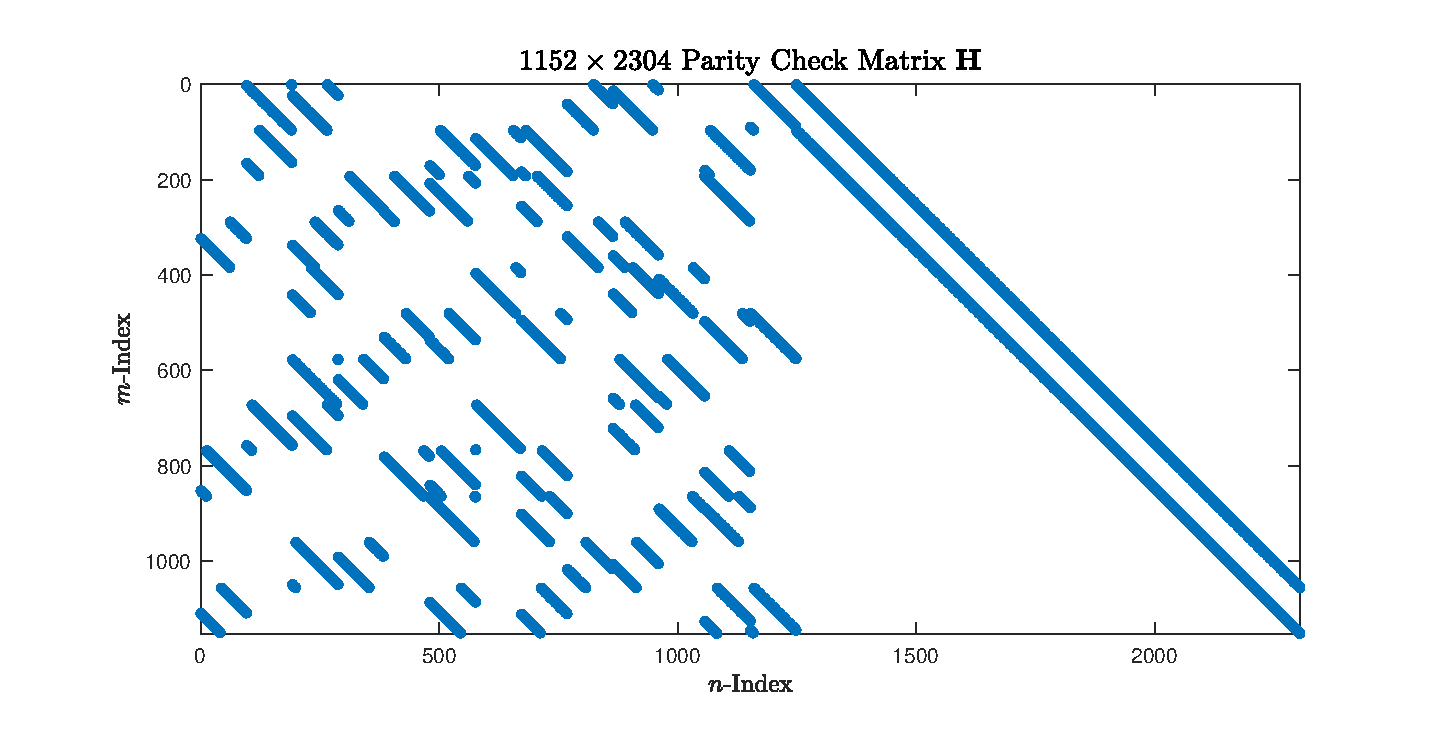
\includegraphics[width=1.25\textwidth, keepaspectratio]{H.eps}
		}
		\caption{Sparsity visualization of the parity-check matrix ${\mathbf{H}}$.}
		\label{fig:hmatrix}
	\end{figure}
	
	
	It is important to notice the $\mathbf{H}$ matrix is large but sparse. Hence, we must devise smart ways to work with it. It is common to implement it as an \verb|.alist| file. In case however, we simply utilize a text file and save the entries with ``1'''s to the text file. This is done both check-node-wise (rows) and variable-node-wise (columns). In the encoding process, we only utilize the check-node-based H matrix in the file \verb|positions_cn_vn.txt|. The encoding process is elaborated in the following section.	

		
	\section{Dual Diagonal Encoding}
	It is a general principle error correction coding to favour systematic encoding, moreso when it can be done efficiently. The key idea in our LDPC encoding is to calculate the parity bits ${\mathbf p} \in GF(2^m), \: m = 1152$, which are be appended to the message bits to form a codeword. This is known as systematic encoding. Although our ${\mathbf H}$ is not in the typical systematic form, it has a special dual diagonal structure, as observed from figure \ref{fig:hmatrix}. Here, we prove this dual diagonal structure from columns $1249 \to 2304$ across all $1152$ rows, can enable systematic encoding via efficient calculation of the parity bits \cite{double_diag}. To prove this, we proceed with the following proof:
	 
	Let $\mathbf{u} = [\mathbf{u}_1, \dots, \mathbf{u}_{12}]$ be a message consisting of 1152 bits. We wish to compute the systematic codeword $\mathbf{c} = [\mathbf{u} \mid \mathbf{p}]$, where $\mathbf{p} = [\mathbf{p}_1, \dots, \mathbf{p}_{12}]$ is the vector of parity bits.
	
	\subsection*{Setup}
	Our systematic LDPC code with parity-check matrix $\mathbf{H} = [\mathbf{H}_m \mid \mathbf{H}_p]$ where $\mathbf{H}_m$ is $m \times m$ and $\mathbf{H}_p$ is $m \times m)$ with dual-diagonal structure as shown in figures \ref{fig:base_matrix} and \ref{fig:hmatrix}.
	
	For message array $\mathbf{u}$, find parity array $\mathbf{p}$ such that codeword $\mathbf{c} = [\mathbf{u} \mid \mathbf{p}]$ satisfies $\mathbf{H}\mathbf{c}^\mathrm{T} = \mathbf{0}$.
	
	\subsection*{Algorithm and Proof}
	\begin{enumerate}
		\item [$\blacksquare$] \textbf{Step 1: Syndrome Calculation}.
		\begin{equation}
			\mathbf{s} = \mathbf{H}_m \mathbf{u}^\mathrm{T}
		\end{equation}
		
		\item [$\blacksquare$] 	\textbf{Step 2: First Parity Block}.
		Using block summation (XOR) over circulant structure:
		\begin{equation}
			\mathbf{p}_0[j] = \bigoplus_{i=0}^{B-1} \mathbf{s}[iZ + j], \quad j = 0, \ldots, Z-1
		\end{equation}
		where $B = 12$ blocks and $Z = 96$ block size.
		
		\item [$\blacksquare$] \textbf{Step 3: Sequential Parity Calculation}.
		For remaining parity bits $p_k$ where $k \geq Z$:
		\begin{equation}
			p_k = \bigoplus_{j: H_{r,j}=1, j < k+n-m} c_j
		\end{equation}
		where $r$ is the row corresponding to parity bit $p_k$.
		
		
	\end{enumerate}
	
	

	\subsection*{Correctness}
	
	The algorithm produces valid codewords since for any parity check equation $i$:
	\begin{align}
		\sum_{j=0}^{k-1} H_{i,j} u_j + \sum_{j=k}^{n-1} H_{i,j} p_{j-k} &= s_i + \sum_{j=k}^{n-1} H_{i,j} p_{j-k}
	\end{align}
	
	By construction:
	\begin{itemize}
		\item Block summation ensures first $Z$ equations are satisfied
		\item Sequential calculation ensures remaining equations are satisfied
	\end{itemize}
	
	Therefore: $\mathbf{H}\mathbf{c}^T = \mathbf{0}$ in $GF(2)$. $\square$
	
	The algorithm achieves $O(n \cdot d_c)$ complexity where $d_c$ is average check node degree, avoiding matrix inversion while maintaining systematic encoding. More detail on complexity is provided in section 5.3.
	
	
	\chapter{Channels}
	\section{BPSK over BI-AWGNC}
	Modulation schemes convert binary sequence sets to channel-ready. In our simulation, we only implement BPSK, which simply maps input bits $ u_j \in \left\{0, 1 \right\} $ to $x_j \in \left\{\pm 1 \right\}$. Several other modulation schemes also exist, BPSK is foundational and regardless of the order of modulation as is the case for QPSK, 16-QAM etc. These would map to different signals for transmission. BPSK is convenient for our simulation since it provides maximum phase separation of $2\pi$, improving channel reliability and easily hard-decision decoding.
	 
	Using inputs from BPSK, the BI-AWGNC channel is modelled as
	$$ y_j = x + n_j, \: n_j \sim \mathcal{N}(0, \sigma^2) \text{ and } x = \left\{ \pm 1 \right\}, \: j = 1, \ldots, n.$$
	Recall $n = 2304$ and the noise is gaussian distributed. We use a zero mean gaussian distribution for simplicity.
	
	Due to our usage of BPSK, $\sigma^2$ and the SNR $\dfrac{E_b}{N_0}$ share the following relation (note that since the code rate is 1/2, the $\text{message length} = m$) 
	\begin{align}
		m E_b= n E_{s} &= \frac{ \mathbb{E} \left[x_j^2\right]}{r} \\
		\Rightarrow \frac{E_b}{N_0} &= \frac{1}{2 r \sigma^2} \\
		\Rightarrow \sigma^2 &= \frac{1}{2 r} \cdot \frac{1}{E_b/N_0}
	\end{align}
	where the first equality is the input-output relation of the encoder for which the message of size $m$ goes in, and encoded symbols of size $n$ goes out into the channel. This is precisely the formula used to for providing the $\sigma^2$ parameter for the \verb|Channel| and \verb|Decoder| classes. Note $r = \frac{m}{n} = \frac{1}{2}$ is our code rate.
	
	\chapter{LDPC Decoding}
	\section{Log Sum Product Algorithm}
	
	Due to the large nature of the ${\mathbf H}$ matrix for storing and handling in C++, we tend to efficient representions. For the implementation accompanying this report, 2 \verb|.txt| files are created for storing the node node connectivity information (position of ones for each row) and vice versa. We utilize these \verb|positions_cn_vn.txt| and \verb|positions_vn_cn.txt| files in the encoding and decoding processes for parity check calculations and tanner graph traversing respectively. Therefore, simulation for each $E_b/N_0$ value keeps utilizes both files 
	
	Following the BI-AWGNC channel model, the received noisy symbol $y_j$ is gaussian distributed. The decoder is initialized by setting all VN messages $L_{j\to i}$ equal to:
	
	\begin{align*} L_j = L(v_j \mid y_j) &= \log \left( \frac{\Pr(v_j = 0 \mid y_j)}{\Pr(v_j = 1 \mid y_j)} \right) = \log \left( \frac{\Pr(x_j = +1 \mid y_j)}{\Pr(x_j = -1 \mid y_j)} \right) \\ 
		& = \log \left( \frac{\left(1 + \exp\left(-\frac{2 y_j }{\sigma^2}\right)\right)^{-1}}{\left(1 + \exp\left(\frac{2 y_j }{\sigma^2}\right)\right)^{-1}} \right)
		= \log \left( \frac{1 + \exp\left(\frac{2 y_j }{\sigma^2}\right)}{1 + \exp\left(-\frac{2 y_j }{\sigma^2}\right)} \right) \\
		&= \log \left( \exp\left(\frac{2 y_j }{\sigma^2}\right)  \cdot \frac{1 + \exp\left(\frac{2 y_j }{\sigma^2}\right)}{1 + \exp\left(\frac{2 y_j }{\sigma^2} \right)} \right) = \frac{2 y_j }{\sigma^2}
	 \end{align*}
	according to the MAP estimation criterion.
	
	It is critical to note that the LDPC code's $\mathbf{H}$ matrix can be regarded as a tanner (also bipartite) graphs, wherewith can apply belief propagation, sharing the soft information across check nodes and variable nodes (message passing). The received likelihood information becomes the message initialization for the variable nodes, to be sent to the check nodes.
	
	To pass information between variable and check nodes, we create several arrays that keep track of the neighours of each node and its connectivity information (the number of edges connected to it). The neighbours refer to the ($\mathbf{H}$ matrix entries) connected to the specified check or variable node (row and column respectively). The other 2 2-d arrays, dubbed \verb*|L_ij| and \verb*|L_ji| of dimensions $m\times10$ and $n\times10$ are used for saving the message passed to the check nodes and variable nodes respectively. We note that the connectivity of each node does not exceed 10, in fact, it is often $\leq 7$. Eitherway, we apply array indexing techniques to avoid needless indexing by utilizing the arrays storing the connectivity \verb|cn_degrees| and \verb|vn_degrees|. These node information are directly obtained from the accompanying \verb|.txt| files which, which serve as a more compact representations of the parity check matrix. 
	
	The check node update is performed using the $\phi(\cdot)$ function and the $\alpha_{ji}$, defined as follows:
	
	\begin{align*}
		L_{j \rightarrow i} &= \alpha_{ji} \beta_{ji}, \\
		\alpha_{ji} &= \operatorname{sign}(L_{j \rightarrow i}), \\
		\beta_{ji} &= \lvert L_{j \rightarrow i} \rvert,
	\end{align*}
	
	
	\begin{equation}\label{eqn:phi_func}
	\phi(x) = -\log[\tanh(x/2)] = \log\left(\frac{e^x + 1}{e^x - 1}\right), \quad x > 0
	\end{equation}
	
	The above expressions are realized in the \verb|phi_func()| function, which plays a critical role in the log SPA decoder.
		\begin{algorithm}
		\caption{The log Sum--Product Algorithm \cite{book_shu_lin} } \label{alg:alg_log_spa}
		\begin{algorithmic}[1] 
			\State \textbf{Initialization:} For all $j$, initialize $L_j$ according to the channel model. For all $i, j$ such that $h_{ij} = 1$, set $L_{j \to i} = L_j = {\dfrac{2 y_j}{\sigma^2}}$.
			
			\State \textbf{CN update:} For each check node $i$ and all $j \in N(i)$:
			\[
			L_{i \to j} = \prod_{j' \in N(i) \setminus \{j\}} \alpha_{j'i} \cdot \phi \left( \sum_{j' \in N(i) \setminus \{j\}} \phi(\beta_{j'i}) \right),
			\]
			
			%\[
			%L_{i \to j} = 2 \tanh^{-1} \left( \prod_{j' \in N(i) \setminus \{j\}} \tanh\left( \frac{1}{2} L_{j' \to i} \right) \right)
			%\]
			
			\Statex Transmit $L_{i \to j}$ to the variable nodes.
			
			\State \textbf{VN update:} For each variable node $j$ and all $i \in N(j)$:
			\[
			L_{j \to i} = L_j + \sum_{i' \in N(j) \setminus \{i\}} L_{i' \to j}
			\]
			
			\Statex Transmit $L_{j \to i}$ to the check nodes.
			
			\State \textbf{LLR total:} For all $j = 0, \dots, n{-}1$, compute:
			\[
			L^{\text{total}}_j = L_j + \sum_{i \in N(j)} L_{i \to j}
			\]
			
			\State \textbf{Stopping criteria:} For each $j = 0, \dots, n{-}1$, set:
			\[
			\hat{v}_j = 
			\begin{cases}
				1 & \text{if } L^{\text{total}}_j < 0 \\
				0 & \text{otherwise}
			\end{cases}
			\]
			
			\State Compute $\mathbf{0} = \hat{\mathbf{c}} \mathbf{H}^\top$. If result is $\mathbf{0}$ or iteration limit = 20 is reached, \textbf{stop}; else, go to Step 2.
		\end{algorithmic}
	\end{algorithm}
	
	These functions come about due to the parity check requirement on the check nodes. Each check node acts as a Single-Parity-Check code, from which we obtain the the CN update equation that is simplified to the one in algorithm \ref{alg:alg_log_spa} \cite{book_shu_lin, qc-ldpc}.
	
	The VN update follows a follows a simply message gathering strategy from the check nodes. This is because it collects messages relevant to detection bits are assumed to be independent, hence, the only goal for the VN update round is to aggregate messages relevant for correct hard-decision decoding. This is similarly realized within our \verb|Decoder| class, first aggregating information from all neighbours and then updating each \verb|L_ji| value after subtracting the pertaining \verb|L_ij|.
	
	Before hard-decision making, the total LLR from all neighbours to the variable node is aggregated and then hard-decisions are made according  to the modulation mapping and likelihood message information.
	
	Finally, it is critical to verify if the decoded codeword is valid. as shown in step 6, otherwise, the procedure continues from step 2 until maximum number of iterations 20 is reached for each codeword.
	
	\section{Minsum Algorithm}
	
	In this section, a basic minsum algorithm is implemented. The motivation here is to show that an approximation of the above log SPA algorithm often leads to faster but less accurate decoders, although the performance must be acceptable for all practical purposes. The goal is to speed up the single-parity-check evaluation of messages. We only consider the simple approximation case, stemming from the properties of the $\phi (\beta_{j'i})$ function. Therefore, the only difference between the minsum approximation decoder and the log SPA is the
	
	\begin{equation} \label{minsum_update} \textbf{CN update: } L_{i \to j} = \prod_{j' \in N(i) \setminus \{j\}} \alpha_{j'i} \cdot \min_{j' \in N(i) \setminus \{j\}} \beta_{j'i}. \end{equation}
	
	The above CN approximation can be proven by considering the properties of the $\phi(\cdot)$ function defined in \ref{eqn:phi_func}. First, it is useful to visualize the function as follows:
	
	\begin{figure}[htbp]
		\centering
		\begin{minipage}[c]{0.55\textwidth}
			\centering
			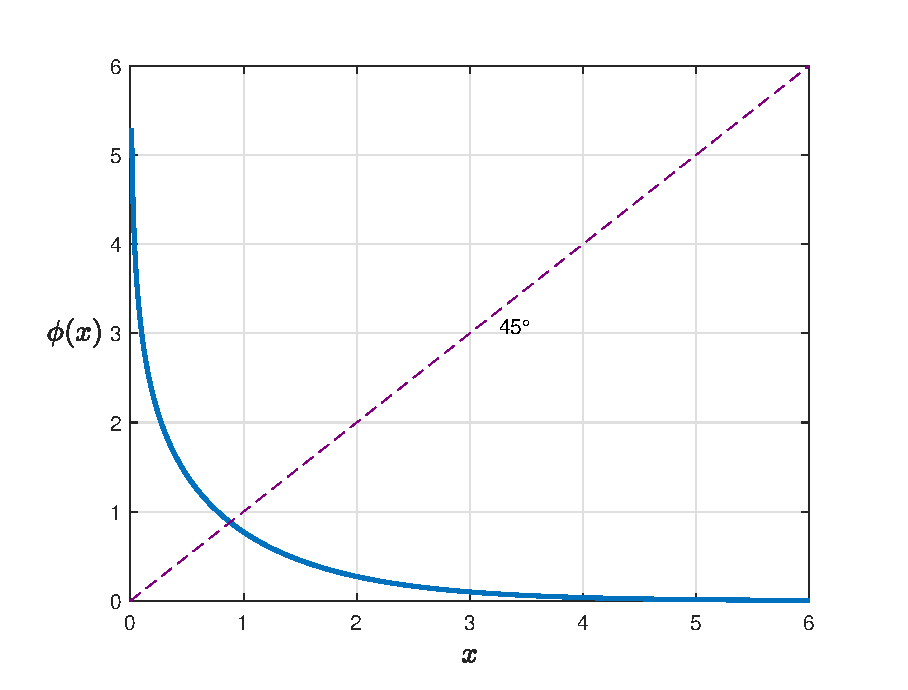
\includegraphics[width=\linewidth,height=0.35\textheight]{phi_func.eps}
			\caption{ $\phi(x)$ function}
			\label{fig:phi_func}
		\end{minipage}%
		\hfill
		\begin{minipage}[c]{0.45\textwidth}
			
			Observing the nature of the $\phi (x)$ function, we can observe that it diminishes exponentially, is symmetric and self-inverse \cite{book_shu_lin}. As a result, we can estimate 
			
			\[ \phi (x_1) + \phi (x_2) + \ldots + \phi (x_n) \simeq \phi (\max_{i = 1,\ldots,n} x_i ) .\]
			
			Consequently, we can also apply the self-inverse property and our CN update equation can be modified as
			\begin{align*}
			\phi\left( \sum_{j'} \phi(\beta_{j'i}) \right) &\simeq \phi\left( \phi\left( \min_{j'} \beta_{j'i} \right) \right) \\
			&= \min_{j' \in N(i) \setminus \{j\}} \beta_{j'i}.
			\end{align*}
			
			This directly leads us to the updated CN update provided in equation \ref{minsum_update}, alongside sign evaluation.
		\end{minipage}
	\end{figure}
	We can observe minsum significantly cuts down the computation involved with \verb|phi_func()|, reducing the complexity of the check node update in the SPA decoder from $\mathcal{O}(m\cdot d_c^2)$ to $\mathcal{O}(m\cdot d_c)$, moreso without factoring the non-linear computations for the \verb|exp()| and \verb|log| functions in C++.
	Another advantage minsum offers is that there is no need for the decoder to utilize the channel noise variance, $\sigma^2$. This is because this estimated positive constant will have no effect on the sign nor on the minimum value selected. Hence, minsum eliminates the need for channel estimation in the decoding process. In our implementation, we utilize sigma anyway, but the results are unchanged when it is removed. Everything else about the simulation stays the same as for the log SPA implementation.
	 
	\chapter{Results and Discussion}
	\section{BER Performance}
	
	We expect our implemented decoder to perform better decoding as the SNR increases. For each SNR value, we randomly generate a large number of message bits, encode them into codewords, transmit over a BI-AWGNC and then decode using the pertaining algorithms. The message part of the decoded codeword is extracted and the total number of bit errors is calculated as follows:
	\[ \text{error rate} = \frac{\text{ sum of total errors}}{ \text{accumulated message size} } \]
	For each SNR, the same process is repeated over multiple rounds and the total message errors are accumulated, alongside the total number of bits transmitted, until convergence is achieved using a 95\% interval for the moving average BER. These are realized within the \verb|BERSimulator| and \verb|StatisticsTracker| classes. Both serve as important helper functions for the overall simulation.
	
	Having obtained the BER values at convergence for each simulated SNR (EbN0) value, we can observe the waterfall trend of the BER curve. The number of simulation errors, and convergence rate of the code significantly increases with increasing BER, achieving up to $\sim 10^{-7}$ for 2.2 dB.
	
	\begin{figure}[H]
		\makebox[\linewidth][c]{%
			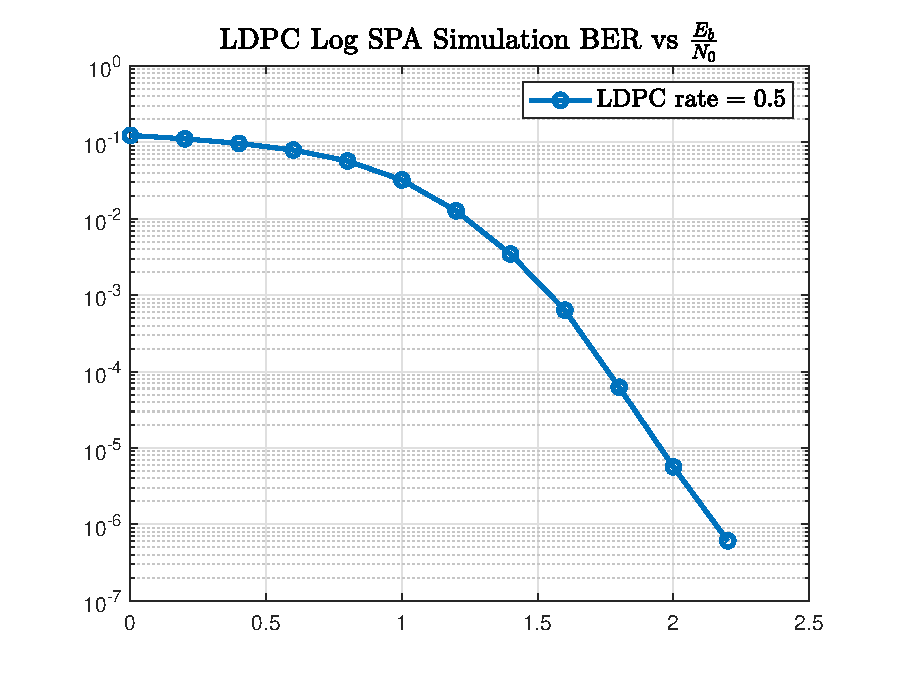
\includegraphics[width=\textwidth, height=0.4\textheight, keepaspectratio]{BER_curve_log_SPA.eps}
		}
		\caption{Log SPA BER Performance Curve}
		\label{fig:ber_logspa}
	\end{figure}
	
	 It is important to note that for the high SNR value 2.2 dB, convergence is hard to achieve due to very few errors encountered. As such, we add a relaxed convergence constraint such that beyond $\sim 10^7$ bits simulated, the current BER becomes the final. In other experiments, we also increase the number of errors required for relaxed convergence to 100 (reasonable number), and run the 2.2 dB point alone, to obtain a more credible value. We settle on the corresponding BER value in the table herein, as appropriate.
	 
	 In reality, there are $2^{1152}$ valid codewords. This is an incredible number which is virtually impossible to iteratively simulate through. Monte carlo methods as applied in this project, therefore provide an appropriate approach to reasonably estimate the BER points.
	 
	\section{BER Performance of Minsum vs Log SPA}
	The minsum vs Log SPA figure follows a similar trend to \ref{fig:ber_logspa}. The minsum decoder shows a degraded BER performance since it is an approximation of log SPA. It is however important to note that this can be improved using other versions of minsum approximation such as attenuated and offset minsum decoders. In addition, we can observe that the minsum decoder is approximately an order of magnitude above the log SPA counterpart, up to approximately 1 dB worse.
	
	\begin{figure}[H]
		\makebox[\linewidth][c]{%
			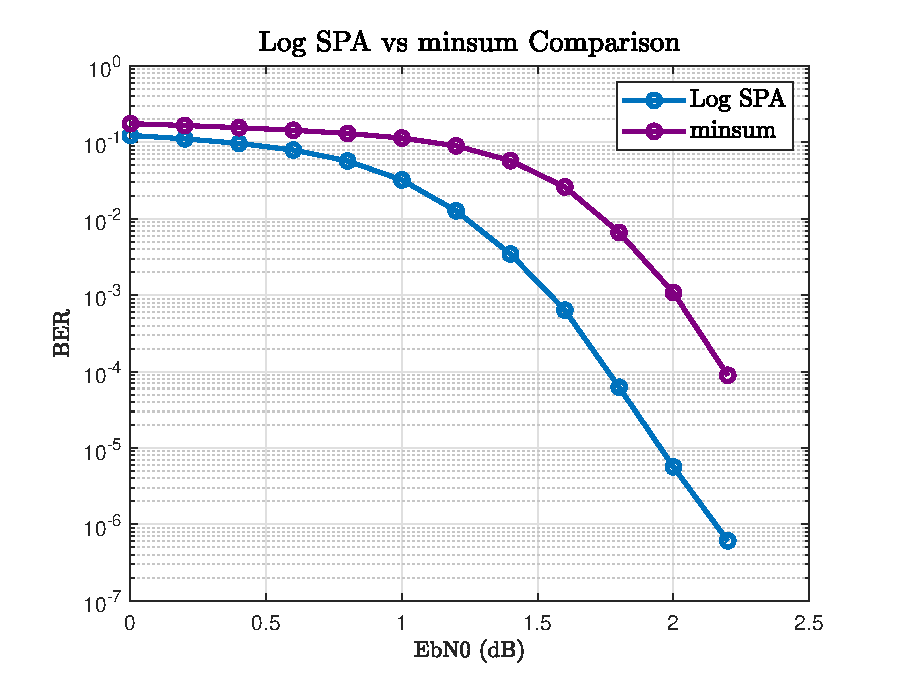
\includegraphics[width=\textwidth, height=0.4\textheight, keepaspectratio]{BER_curve_log_SPA_vs_minsum.eps}
		}
		\caption{Log SPA vs minsum BER Curve}
		\label{fig:ber_logspa_vs_minsum}
	\end{figure}
	
	The following table \ref{tab:table-pts} displays the BER values of both simulations, with more details including number of errors and number of bits simulated until converged value, provided in the excel sheet \verb |simulation_results.xlx|.
	\begin{table}[H]
		\centering
		\caption{BER Results Log SPA and Min-Sum Algorithms}
		\label{tab:table-pts}
		\begin{tabular}{|c|c|c|}
			\hline
			$\mathbf{E_b/N_0}$ \textbf{(dB)} & \textbf{BER: Log SPA} & \textbf{BER: minsum} \\
			\hline
			0.0 & 1.230e-01 & 1.752e-01 \\
			0.2 & 1.109e-01 & 1.658e-01 \\
			0.4 & 9.672e-02 & 1.551e-01 \\
			0.6 & 7.907e-02 & 1.435e-01 \\
			0.8 & 5.682e-02 & 1.304e-01 \\
			1.0 & 3.209e-02 & 1.136e-01 \\
			1.2 & 1.264e-02 & 8.966e-02 \\
			1.4 & 3.440e-03 & 5.737e-02 \\
			1.6 & 6.371e-04 & 2.602e-02 \\
			1.8 & 6.226e-05 & 6.601e-03 \\
			2.0 & 5.660e-06 & 1.077e-03 \\
			2.2 & 6.097e-07 & 8.950e-05 \\
			\hline
		\end{tabular}
		\label{tab:ber_minsum}
	\end{table}
	
	
	\section{Complexity analysis}
	Here, we provide complexity analysis of the encoder and decoder algorithms implemented. We also compare the implementation complexity of the minsum algorithm as specified in the section 4.2 with log SPA. We find that minsum indeed runs faster due to the reduced complexity. First,
	
	\begin{enumerate}
		\item \textbf{Encoder}. The encoder is precisely the same for both the log SPA and minsum algorithm. Our implemented algorithm takes $\mathcal{O} (m \cdot d_c) +  \mathcal{O} (m) + \mathcal{O} (1056 \cdot d_c)$, corresponding to syndrome calculation, first parity block calculation (96 bits) and remaining parity bits calculation respectively. 
		
		\item \textbf{Decoder} For the log SPA decoder, our implementation takes $\mathcal{O} (m\cdot d_c^2)$ for the CN update, $\mathcal{O} (n\cdot d_v^2)$ for the VN update, $\mathcal{O} (n\cdot d_v^2)$ for the total LLR and $\mathcal{O} (m\cdot d_c)$ for the stopping criterion.
		
		\item \textbf{General Simulation Strategy}
		
		For simulation, we apply monte carlo methods to continue calculating the BER until a convergence criterion using confidence intervals is achieved. We use a 95\% confidence interval. This overall slows down the simulation and results in several hours of waiting, however, it helps in the estimation of a somewhat true BER for any given $E_b/N_0$. 
		
	\end{enumerate}
	
	\chapter{Conclusion and Future Work}
	In this project, we have implemented the log SPA algorithm, a belief-propagation-based soft messaging passing algorithm for decoding a $1152 \times 2304$ QC-LDPC code, commonly used in the WiMaX standard. We further modified the decoder to the simple minsum decoder case. As a result, we show that while the minsum decoder has a lower complexity, it is an approximation of the original log SPA algorithm and as a result, it's BER performance degrades. 
	
	For future work, we will consider modifying the \verb|Channel| class to model a BSC channel and a BEC. Consequently, the decoders will be modified to implement the bit-flipping (Gallager's algorithm A) and iterative filling algorithms respectively. We will also consider other mofications to the minsum decoder such as the attenuated and off-set decoders, and other state of the art techniques. This will further build capacity and comfort with working on similar projects in the future. Further studies may also be performed on the construction procedure for irregular LDPC codes, which often entail solving linear optimization problems (relaxed), utilizing the node degree distribution polynomials.
	
	In conclusion, LDPC codes provide incredible performance, achieving very low bit error rates as SNR increases. This are also long codes, making them ground-breaking and suitable for several high speed applications including the recent 5G NR LDPC codes.
	
		\appendix
		\chapter{Monte Carlo Methods and Useful Statistics}
		
		Here, we present the statistical methods and convergence criteria utilized to obtain the BER values in our LDPC simulation. The Monte Carlo simulation employs key parameters to ensure statistical reliability: $1 \times 10^7 \to 2\times 10^7$ minimum information bits per SNR point, $100 \to 200$ minimum errors before convergence assessment, and a maximum of $150,000$ simulation rounds per SNR point. Convergence is assessed every 50 rounds using a statistical window of 100 recent BER observations.
		
		\section*{Statistical Measures and Convergence Detection}
		
		For the sliding window of $n = 100$, recent BER observations $x_1, x_2, \ldots, x_n$, the sample mean is calculated as 
		\[ \bar{x} = \frac{1}{n} \sum_{i=1}^{n} x_i. \] 
		The implementation maintains a circular buffer (vector) where the oldest BER value is replaced with the most recent observation every 50 rounds. The sample variance is also obtained using 
		
		\[ s^2 = \frac{1}{n-1} \sum_{i=1}^{n} (x_i - \bar{x})^2, \] 
		with the sample standard deviation following as $s = \sqrt{s^2}$.
		
		For 95\% confidence interval estimation, we assume the BER samples follow an approximately normal distribution. The confidence interval for the true mean $\mu_{\text{BER}}$ is constructed as:
		
		\[ \mu_{\text{BER}} \in \left[ \bar{x} - z \cdot \frac{s}{\sqrt{n}}, \bar{x} + z \cdot \frac{s}{\sqrt{n}} \right] \]
		where $z = 1.96$ is the critical value for 95\% confidence from the standard normal distribution.
		
		Statistical convergence is declared when the relative half-width of the 95\% confidence interval falls below a specified threshold \cite{stats, yt-video}: 
		
		\[ \frac{1.96 \cdot s/\sqrt{n}}{\mu_{\text{BER}}} < 0.1, \] 
		
		ensuring the confidence interval half-width is within 10\% of the estimated mean BER \cite{yt-video, stats}. Following this, we implement a dual stopping criteria for the BER estimation: primary convergence requires both minimum bits $\sim 10^7$ and errors (200) to be satisfied along with statistical convergence, while a fallback criterion relaxes the error threshold to 50 errors for high SNR scenarios with extended bit counts ($\sim 10^8$ bits).
		
		The simulation uses a fixed seed (42) for reproducibility and generates independent Gaussian noise samples using the \verb|Normal()| function for proper AWGN channel modeling, alongside the calculated channel \verb|sigma| value from section 3.1. Progress monitoring occurs every 200 rounds, displaying current round number, accumulated errors, total bits simulated, and current BER estimate. This statistical framework ensures that reported BER values represent statistically significant estimates with quantified confidence bounds, particularly important for the low BER regime, typical of LDPC codes at moderate to high SNR values.
	
	\begin{thebibliography}{9}
		
		\bibitem{book_shu_lin}
		Ryan, William, and Shu Lin. Channel codes: classical and modern. Cambridge university press, 2009.
		
		\bibitem{double_diag}
		Chia-Yu Lin, Chih-Chun Wei and Mong-Kai Ku, "Efficient encoding for dual-diagonal structured LDPC codes based on parity bit prediction and correction," APCCAS 2008 - 2008 IEEE Asia Pacific Conference on Circuits and Systems, Macao, China, 2008, pp. 1648-1651, doi: 10.1109/APCCAS.2008.4746353.
		
		
		\bibitem{qc-ldpc}
		Hasani, Alireza, Lopacinski, Lukasz, Kraemer, Rolf. (2021). Reduced-complexity decoding implementation of QC-LDPC codes with modified shuffling. EURASIP Journal on Wireless Communications and Networking. 2021. 183. 10.1186/s13638-021-02056-5. 
		
		\bibitem{stats}
		DATAtab: DATAtab Team (2025). DATAtab: Online Statistics Calculator. DATAtab e.U. Graz, Austria. URL \url{https://datatab.net}
		
		\bibitem{yt-video}
		Youtube: Learning OnDemand, (2020), Hypothesis Testing - Hypothesis Testing - Making Decision Using Confidence Interval, URL \url{https://www.youtube.com/watch?v=yuIvN5ETtcI}.
		
		\bibitem{rptu}
		RPTU, ``Channel Codes Database, WiMax LDPC'', [Online]. Available: \url{https://rptu.de/en/channel-codes/channel-codes-database/wimax-ldpc}.
		
	\end{thebibliography}
	


\end{document}
